\section{Tagger Performance} 

\frame{
    \frametitle{ Tagger Performance After Retuning }
    \begin{itemize}
        \item $T \bar T$ MC-Production Used: 
        \begin{tiny} 
            mc16\_13TeV.410470.PhPy8EG\_A14\_ttbar\_hdamp258p75\_nonallhad.
            digit.AOD.e6337\_e5984\_s3126\_r11392\_d1512\_r11391
        \end{tiny}
        \item 4M events total, divided three ways:
        \begin{itemize}
            \item Step 1: 1.5M events
            \item Step 2-3: 1.5M events
            \item Step 4: 1M events
        \end{itemize}
        \item Samples are not cross validated yet (coming soon)
    \end{itemize}

    \begin{table}
    \resizebox{\textwidth}{!}{%
    \begin{tabular}{| l | l | l | l |}
        \hline
        Trigger Title & Input Chain & Track Key & Prm Vtx Key \\
        \hline \hline
        HLT & HLT\_j35\_boffperf\_split & InDetTrigTrackingxAODCnv\_Bjet\_IDTrig & xPrimVx\\
        %FTKVtx & HLT\_j35\_boffperf\_split\_FTKVtx\_L1J15 & InDetTrigTrackingxAODCnv\_Bjet\_IDTrig & PrimVertexFTK\\
        FTK IDTrig & HLT\_j35\_boffperf\_split\_FTK\_L1J15 & InDetTrigTrackingxAODCnv\_Bjet\_FTK\_IDTrig & PrimVertexFTK\\
        %FTK Refit & HLT\_j35\_boffperf\_split\_FTKRefit\_L1J15 & InDetTrigTrackingxAODCnv\_Bjet\_FTKRefit & PrimVertexFTK\\
        \hline
    \end{tabular}}
    \end{table}
}

\frame{
    \frametitle{ IP2D and IP3D Performance } 
    \begin{columns}
        \begin{column}{0.5\textwidth}
            \begin{figure}
                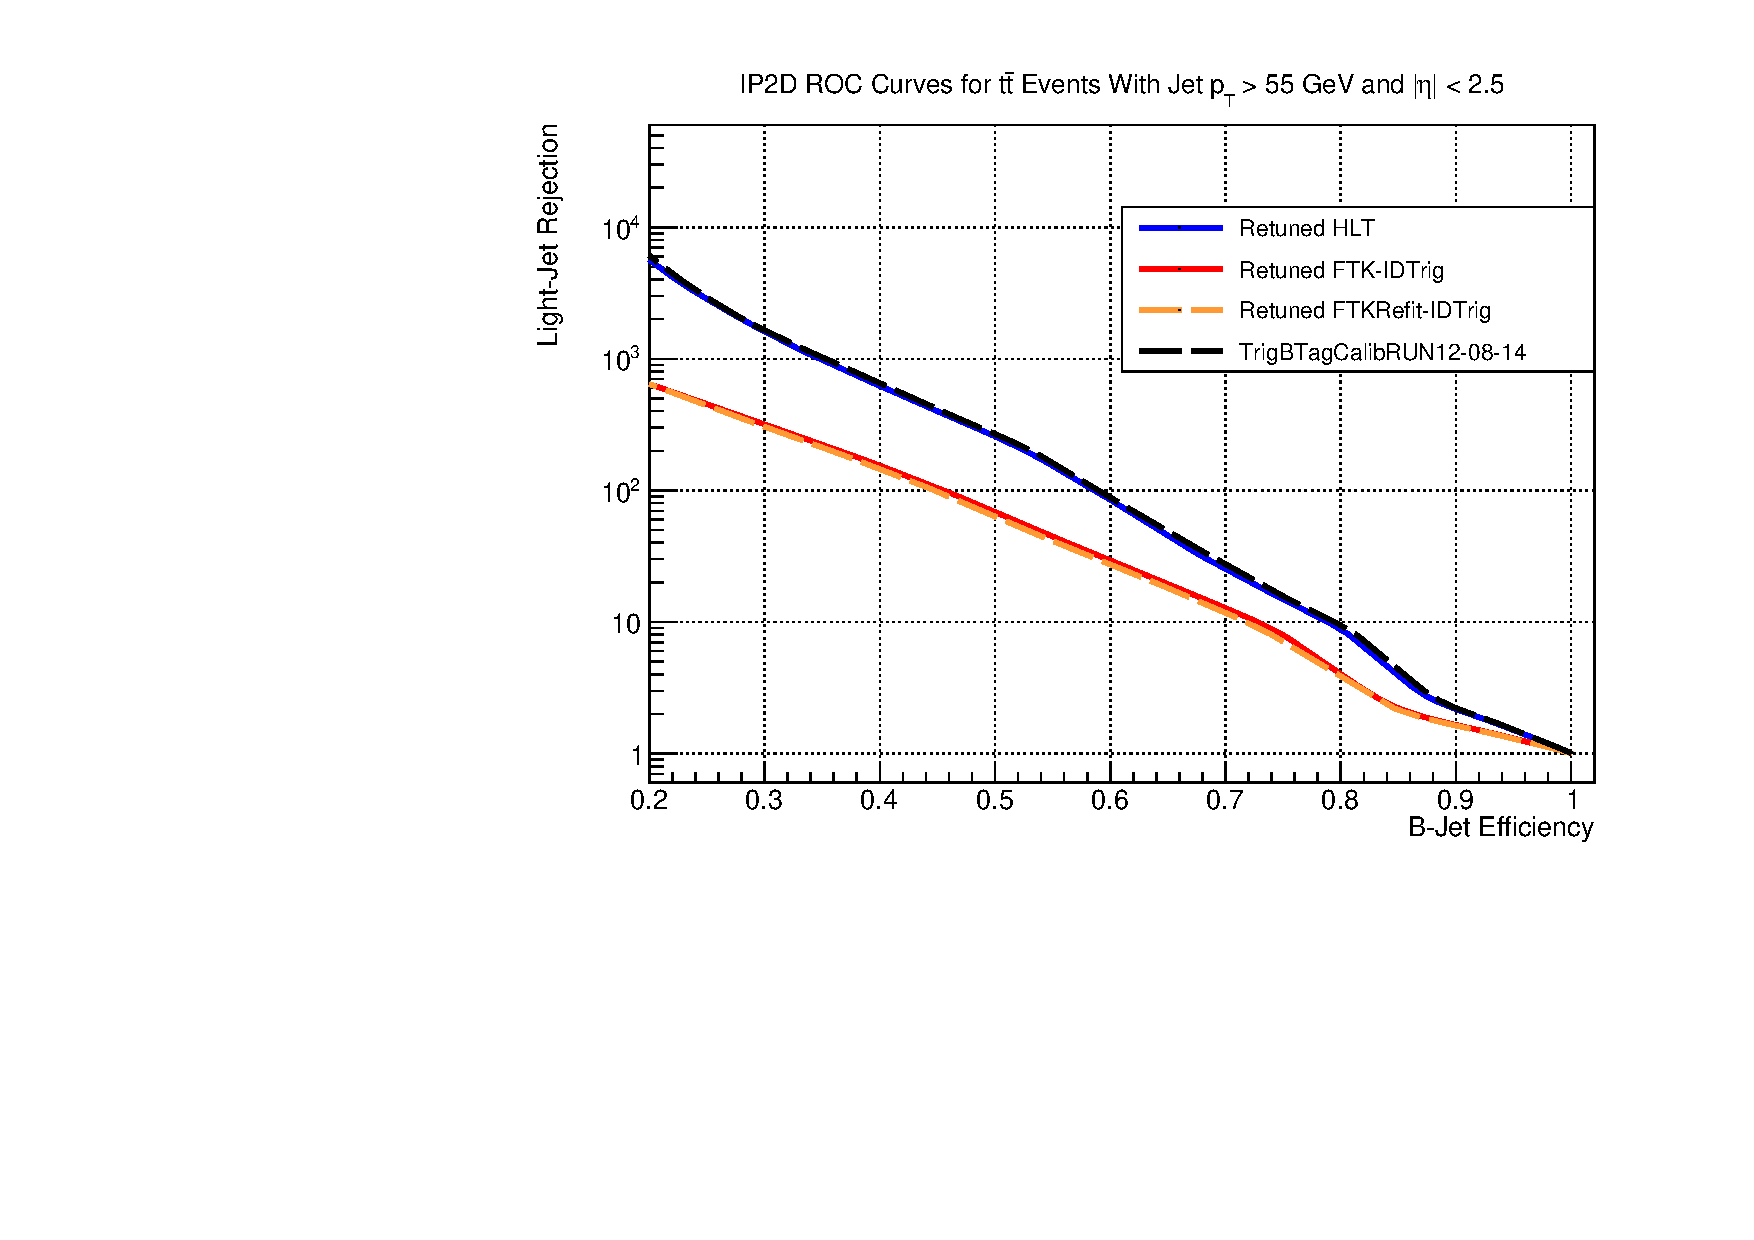
\includegraphics[width=\linewidth,height=\textheight,keepaspectratio]{ipxd_performance/performance_roc_ttbar_ip2d}
            \end{figure}
        \end{column}
        \begin{column}{0.5\textwidth}
            \begin{figure}
                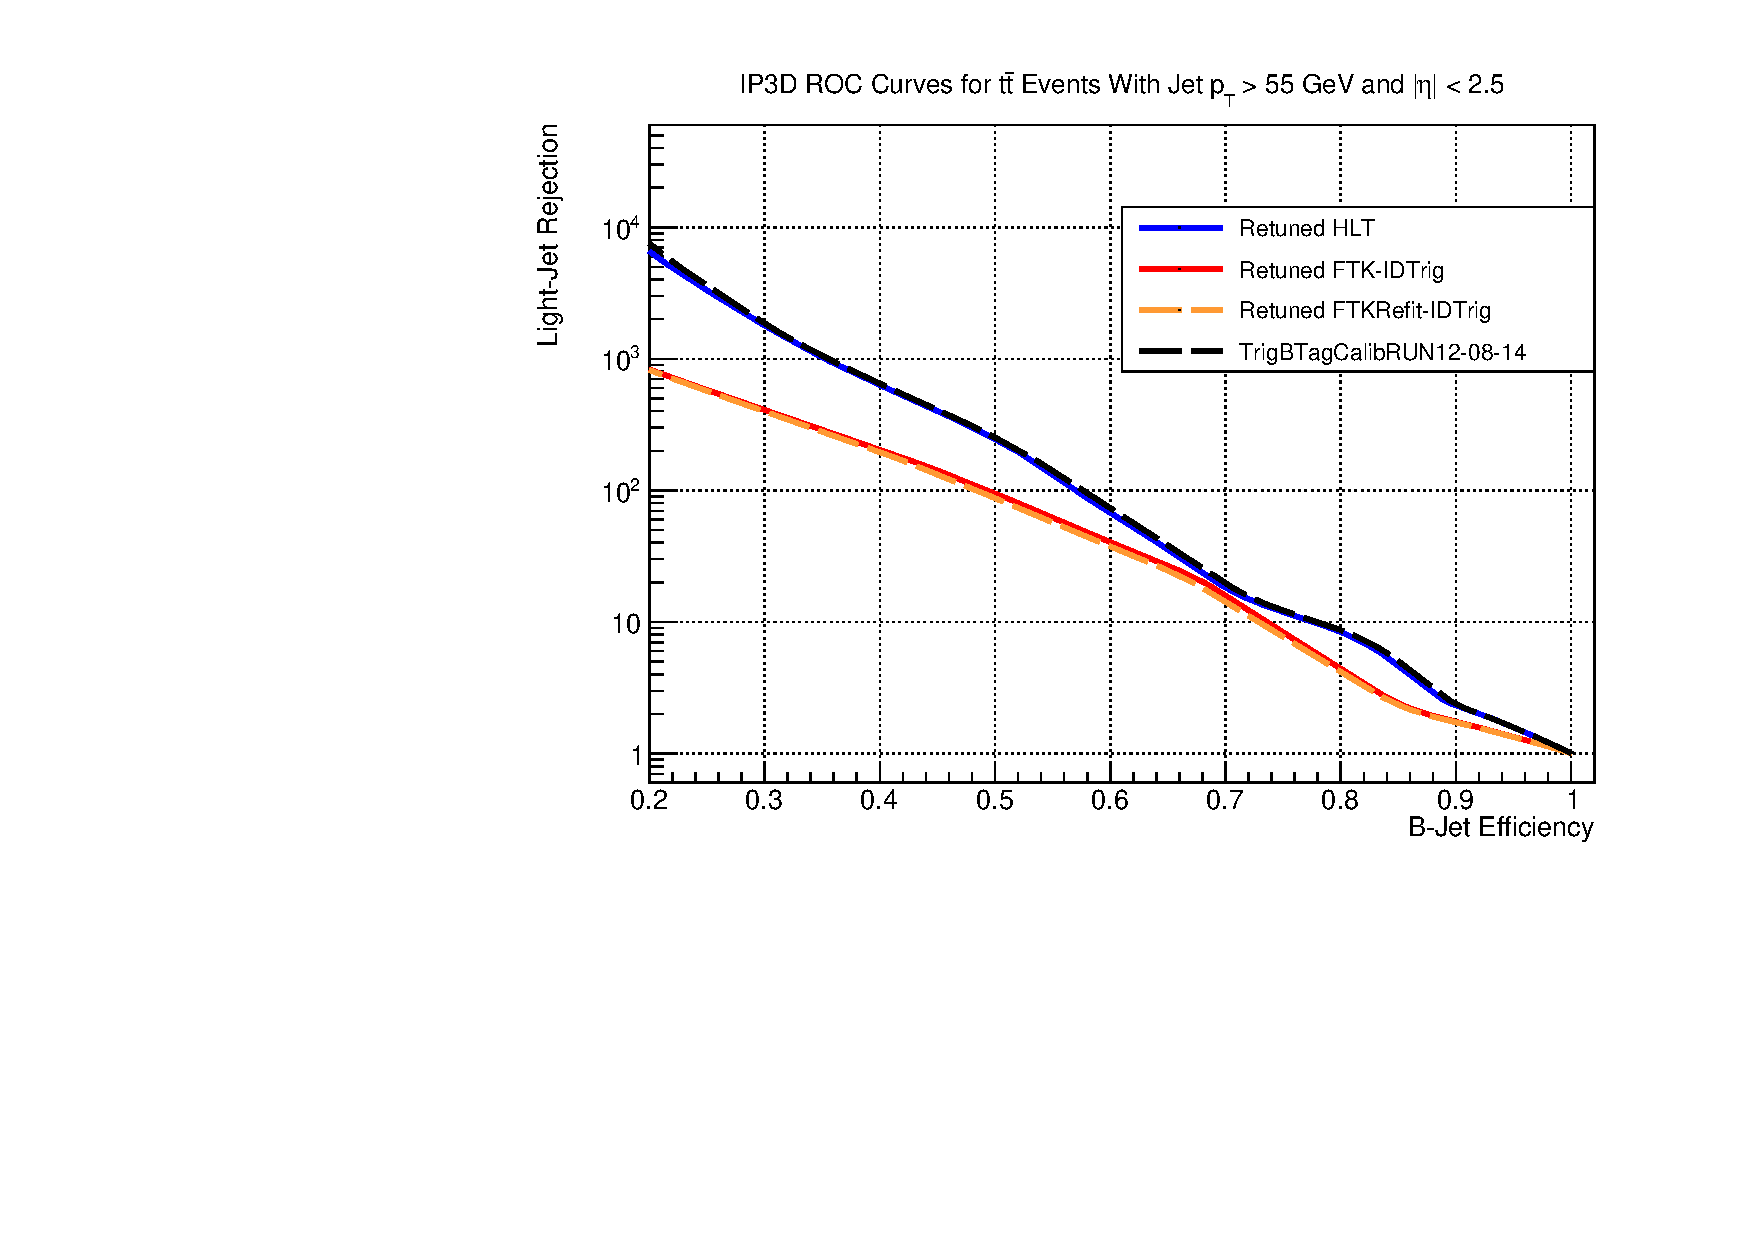
\includegraphics[width=\linewidth,height=\textheight,keepaspectratio]{ipxd_performance/performance_roc_ttbar_ip3d}
            \end{figure}
        \end{column}
    \end{columns}
}

\frame{
    \frametitle{ MV2c10 Performance } 
    \begin{figure}
        \includegraphics[width=\linewidth,height=\textheight,keepaspectratio]{btag_c10_score_comparison/performance_roc_ttbar}
    \end{figure}
}
